\section{Methods}

\begin{figure}[H]
    \centering
    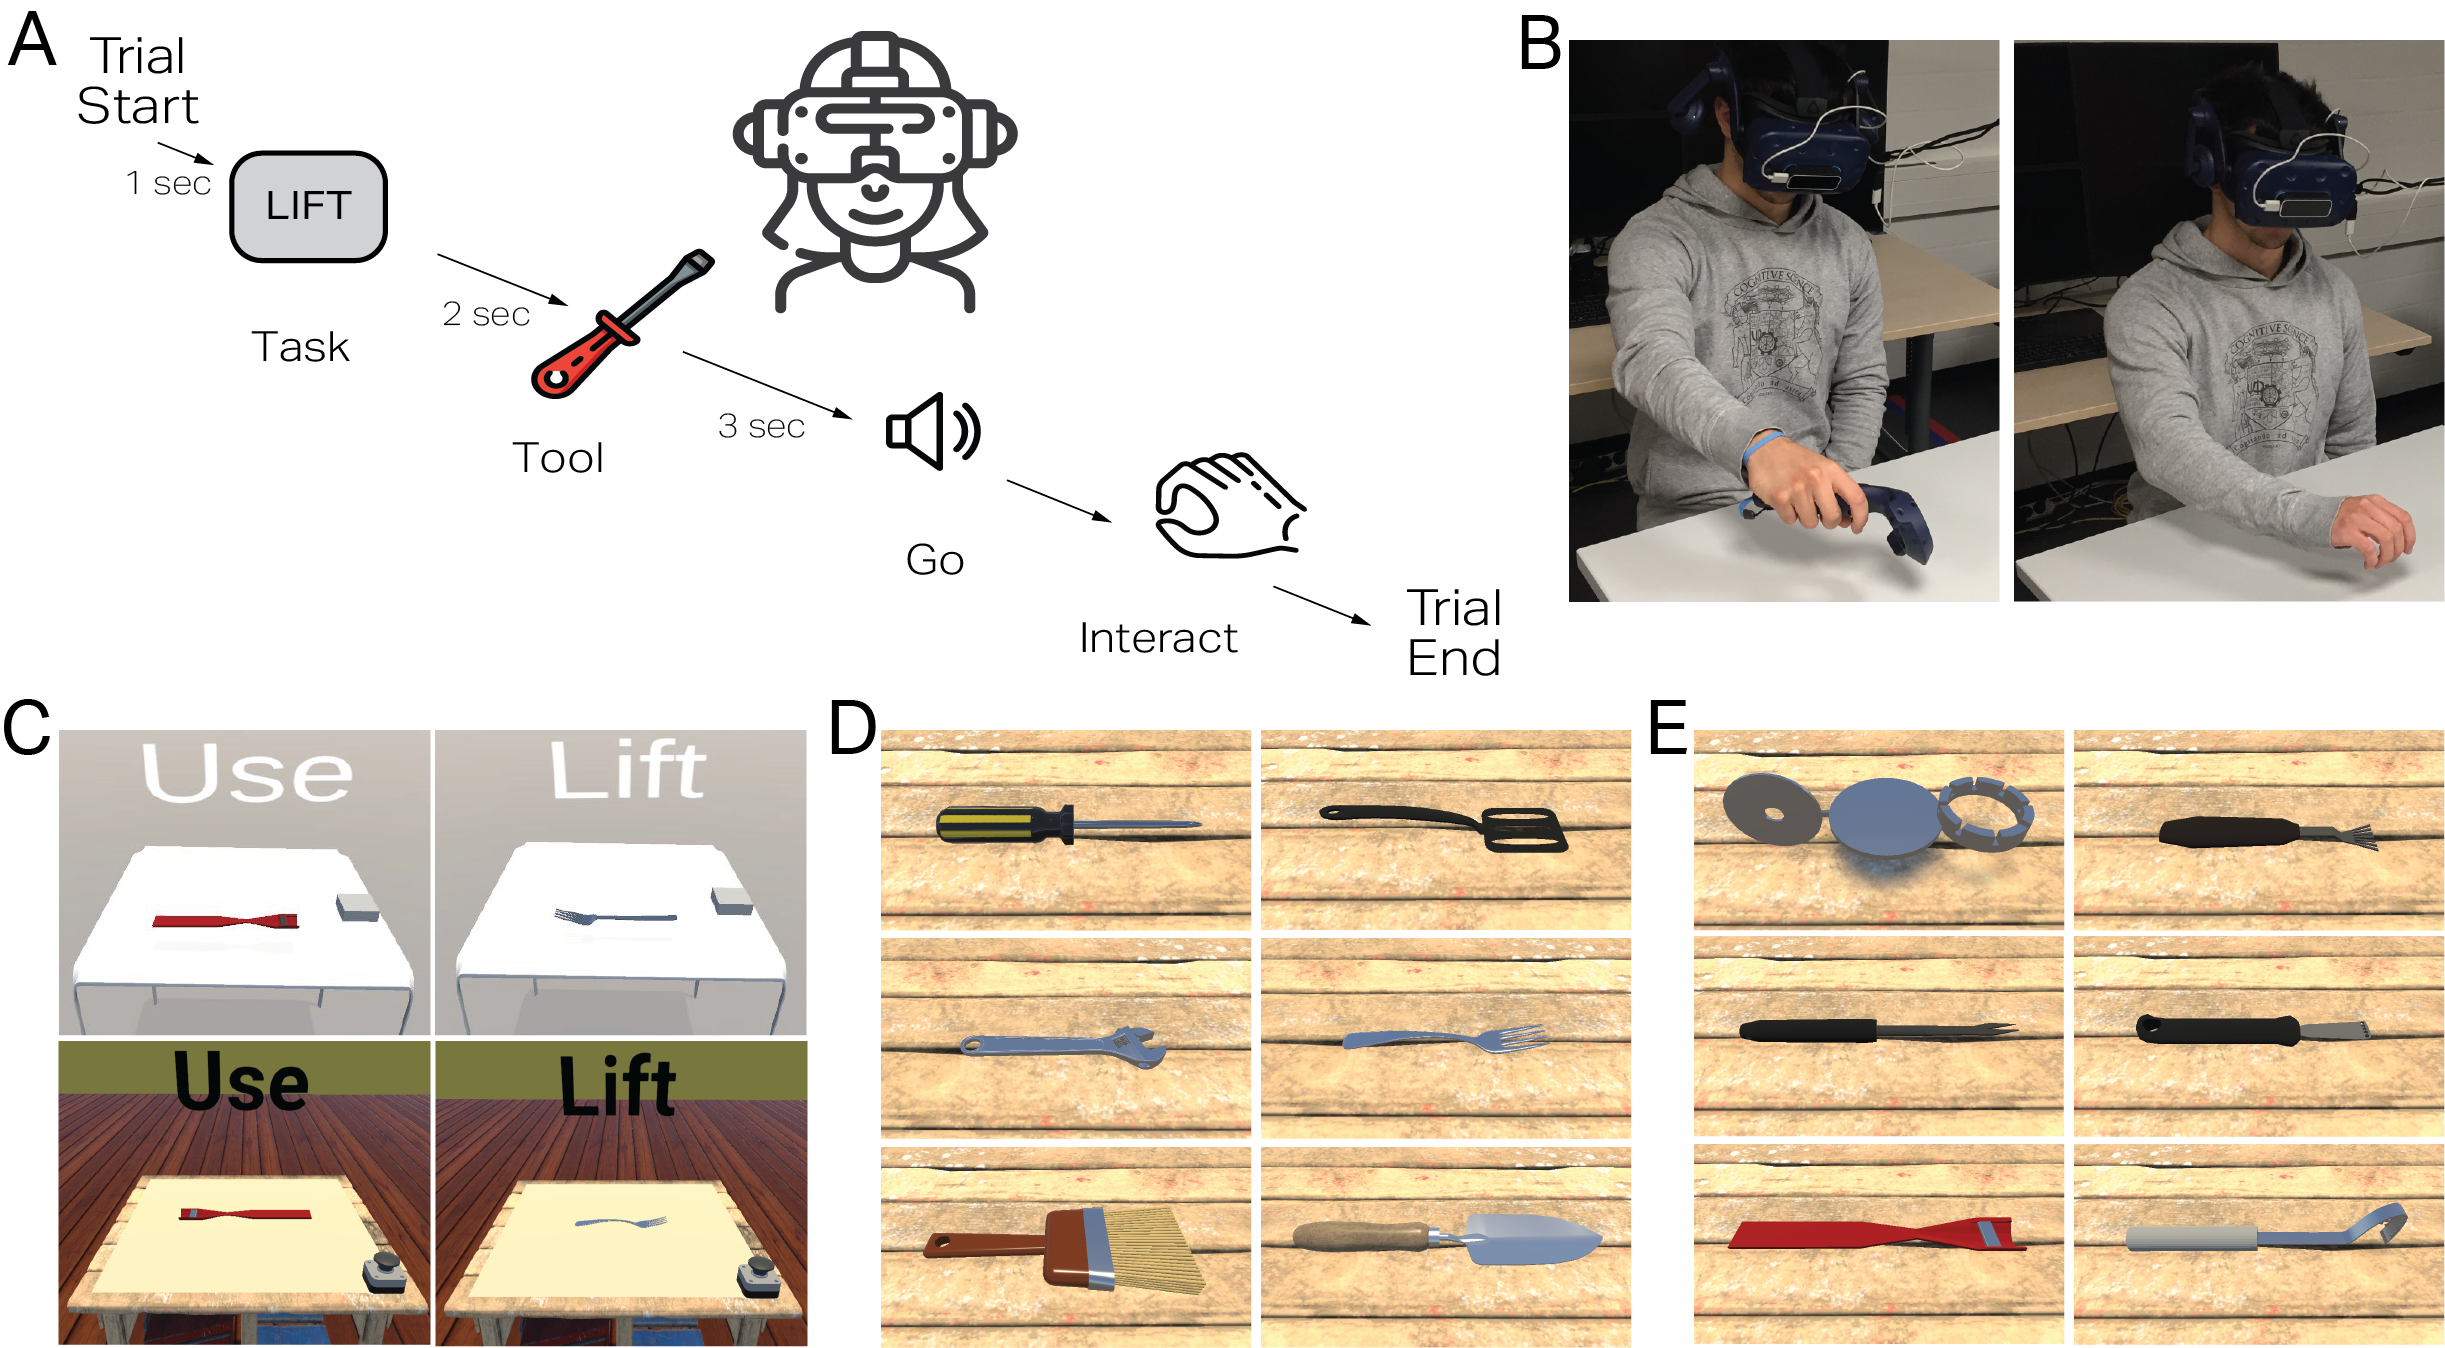
\includegraphics[width=1\linewidth]{source/figures/setup/Methods_1.png} \\
    \caption[]{Experimental Task. In two virtual environments (VEs) participants interacted with tools in two ways (LIFT, USE). The tools were categorized based on familiarity (FAMILIAR, UNFAMILIAR) and were presented to the participants in two different orientations (HANDLE LEFT, HANDLE RIGHT). The two VEs differed based on the mode of interaction where in one experiment, subjects' hand movements were rendered virtually using the VR controllers and in the other the hands were rendered using Leap Motion allowing for more natural view of the hands. Panel \textbf{A} shows the timeline of a trial. Panel \textbf{B} shows a subject in real life performing the task in the two experiments.}
    \label{figure:task}
\end{figure}

\subsection{Participants}

For experiment-I with the interaction method of HTC Vive controller, we recruited a total of 18 participants ( 14 females, mean age = 23.68, SD = 4.05 years). For experiment-II with interaction method using Leap Motion we recruited 30 participants (14 female, mean age=22.7, SD = 2.42 years). All participants were recruited from the University of Osnabrück and the University of Applied Sciences Osnabr{\"u}ck. Participants had a normal or corrected-to-normal vision and no history of neurological or psychological impairments. All of the participants were right-handed. They either received a monetary reward of €10 or one participation credit per hour. Before each experimental session, subjects gave their informed consent in writing. They also filled out a questionnaire regarding their medical history to ascertain they did not suffer from any disorder/impairments which could affect them in the virtual environment. Once we obtained their informed consent, we briefed them on the experimental setup and task. 

% ****This cover has been designed using resources from Flaticon.com

\subsection{Apparatus \& Procedure}
For both experiments, we used an HTC Vive head-mounted display (HMD)(110° field of view, 90Hz, resolution 1080 x 1200 px per eye) with a built-in Tobii  eye-tracker \footnote{\href{https://enterprise.vive.com/us/product/vive-pro-eye/}{https://enterprise.vive.com/us/product/vive-pro-eye-office/}}. The HTC Vive Lighthouse tracking system provided positional and rotational tracking and was calibrated for 4m x 4m space. For calibration of the gaze parameters, we used 5-point calibration function provided by the manufacturer. To make sure the calibration error was less than $1^\circ$, we performed a 5-point validation after each calibration. Due to the nature of the experiments, which allowed a lot of natural head movements, the eye tracker was calibrated repeatedly during the experiment after every block of trials. We designed the experiment using the Unity3D game engine \footnote{\href{www.unity.com}{Unity, www.unity.com}} (v2019.2.14f1) and controlled the eye-tracking data recording using HTC VIVE Eye Tracking SDK SRanipal\footnote{\href{https://developer.vive.com/resources/vive-sense/sdk/vive-eye-tracking-sdk-sranipal/}{SRanipal, developer.vive.com/resources/vive-sense/sdk/vive-eye-tracking-sdk-sranipal/}} (v1.1.0.1)

For experiment-I, we used HTC Vive controller\footnote{\href{https://valvesoftware.github.io/steamvr_unity_plugin/articles/Quickstart.html}{SteamVR, https://valvesoftware.github.io/steamvr\_unity\_plugin/articles/Quickstart.html}} (version 2.5) to interact with the tool. The controller in the virtual environment (VE) was rendered as a gloved hand. When participants pulled the trigger button of the controller with their right index finger, their right hand made a power grasp action. To interact with the tools, subjects pulled the trigger button of the controller over the virtual tools and the rendered hand grasped the tool handle. 

Similarly, in experiment-II, we used LeapMotion\footnote{\href{https://developer.leapmotion.com/unity}{LeapMotion Unity modules, https://developer.leapmotion.com/unity}} (version 4.4.0) to render the hand in the VE. Here, subjects could see their finer hand and finger movements of their real world actions rendered in the VE. When participants made a grasping action with their hand over the virtual tool handle, the rendered hand grasped the tool handle in the VE.

\subsection{Experimental Stimuli}
In both experiments, the experimental setups consisted of a virtual table that mimicked the table in real-world. The height, width and length of the table were 86cm, 80cm, 80cm respectively. In experiment-I, subjects were present in a bare room with grey walls, and constant illumination. They sat before a light grey table, with a dark grey button with which they could indicate the end of the trial. Similarly, In experiment-II, subjects were present in a more immersive, naturalistic room. They sat in front of a wooden desk that had the same dimensions as the real-world table.



\subsection{Experimental Task}
The experimental setup consisted of ... 



\subsection{Data pre-processing}

\subsubsection{Gaze Data}

As a first step, using eye-in-head 3d gaze direction vector for the cyclopean eye we calculated the gaze angles in degrees for the horizontal $\theta\textsubscript{h}$ and vertical $\theta\textsubscript{v}$ directions. All of the gaze data was sorted by the timestamps of the collected gaze samples. The 3d gaze normals are represented as $(x, y, z)$ a unit vector that defines the direction of the gaze in VR world space coordinates. In our setup, the x coordinate corresponds to the left-right direction, y in the up-down direction, z in the forward-backward direction. The formulas used for computing the gaze angles are as follows:

 \begin{equation*}\label{eq:h_angle}
     \theta\textsubscript{h} = \frac{180}{\pi} \arctan{\frac{x}{z}}
 \end{equation*}   
  \begin{equation*}\label{eq:v_angle}
     \theta\textsubscript{v} = \frac{180}{\pi} \arctan{\frac{y}{z}} 
 \end{equation*}   
 
Next, we calculated the angular velocity of the eye in both the horizontal and vertical coordinated by taking a first difference of the angular velocity and dividing by the difference between the timestamp of the samples using the formula below:
\begin{equation*}\label{eq:h_vel_angle}
    \omega\textsubscript{h} = \Delta\theta\textsubscript{h} / \Delta t
 \end{equation*}  
 \begin{equation*}\label{eq:v_vel_angle}
     \omega\textsubscript{v} = \Delta\theta\textsubscript{v} / \Delta t
 \end{equation*}  

Finally, we calculated the magnitude of the angular velocity ($\omega$) at every timestamp from the horizontal and vertical components using:
\begin{equation*}\label{eq:vel_angle}
     \omega = \sqrt{\omega_h^2 + \omega_v^2}
 \end{equation*}  

To filter the samples where gaze was relatively stable, we used an adaptive threshold method for saccade detection described by \citet{Voloh2019-oc}. The schematic of the algorithm used for saccade detection is shown in figure \ref{figure:at_mad}. After this, we calculated the duration of the fixations and removed the fixations that had duration less than 50ms.
% \begin{figure}[H]
%     \centering
%     \includegraphics[width=0.5\linewidth]{source/figures/experiment_setup/saccade_detection.jpg} \\
%     \caption[]{Saccade detection algorithm. As the participants were completely mobile during the experiment, we used an adaptive method to determine the saccade velocity threshold. We selected an initial saccade velocity $\theta\textsubscript{0}$ of $200^\circ$/sec. All eye movement samples with angular velocity less than $\theta\textsubscript{0}$ were used to compute a new threshold $\theta\textsubscript{1}$  using 3 times the median absolute deviation of the selected samples. If the difference between $\theta\textsubscript{0}$ and $\theta\textsubscript{1}$ was less than or equal to $1^\circ$/sec $\theta\textsubscript{1}$ was selected as the saccade threshold, else algorithm was repeated with $\theta\textsubscript{1}$ as the new filtering threshold. The algorithm was repeated until the difference between the $\theta\textsubscript{0}$ and $\theta\textsubscript{1}$ was less than or equal to $1^\circ$/sec.}
%     \label{figure:at_mad}
% \end{figure}

\subsection{Data Analysis}\label{sec:data_analysis}
